\documentclass{article}
\usepackage{layout}
\usepackage[utf8]{inputenc}
\usepackage[a4paper, total={6in, 8in}]{geometry}
\usepackage{graphics}
\usepackage{amsmath}


\graphicspath{ {./src/} }


\headheight=0pt
\title{\textbf{Kinematic calculations for mobile robots using Omni/Meccanum wheels}}
\author{Sujith Christopher}
\date{January 2023}
\begin{document}

\maketitle

\section{Generalized expression}

% refer book
\begin{large}
    This general expression is taken from the book \\
    "Modern robotics mecanics planning and control" by Kevin M Lynch, Frank C Park,
    page no 512, please refer this section for more details.
\end{large}


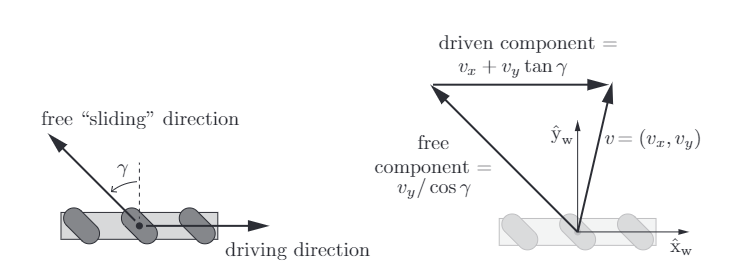
\includegraphics{omni_wheel_kinematics_2.png}
\section{Three wheel omnidirectional robot}
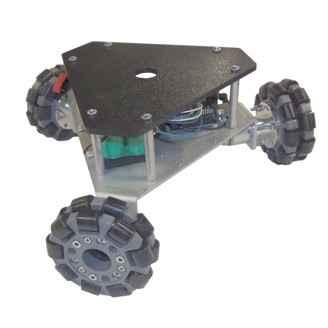
\includegraphics{robot_3_omniwheel.jpg}


\begin{equation}
    h_1(0) \mathcal{V}_b = \frac{1}{r_i} \left[\begin{array}{cc}
            1 & \tan\gamma_i \\
        \end{array}\right]
    \left[\begin{array}{cc}
            \cos \beta_i  & \sin \beta_i \\
            -\sin \beta_i & \cos \beta_i \\
        \end{array}\right]
    \begin{bmatrix}
        -y_i & 1 & 0 \\
        x_i  & 0 & 1 \\
    \end{bmatrix} \mathcal{V}_b
\end{equation}

\begin{equation*}
    \gamma_1 = 0, \beta_1 = 0
\end{equation*}

\begin{equation}
    = \frac{1}{r_1} \left[\begin{array}{cc}
            1 & 0 \\
        \end{array}\right]
    \left[\begin{array}{cc}
            \cos 0  & \sin 0 \\
            -\sin 0 & \cos 0 \\
        \end{array}\right]
    \begin{bmatrix}
        -y_1 & 1 & 0 \\
        x_1  & 0 & 1 \\
    \end{bmatrix}
    \mathcal{V}_b
\end{equation}

\begin{equation}
    = \frac{1}{r_1} \left[\begin{array}{cc}
            1 & 0 \\
        \end{array}\right]
    \begin{bmatrix}
        1 & 0 \\
        0 & 1 \\
    \end{bmatrix}
    \begin{bmatrix}
        -y_1 & 1 & 0 \\
        x_1  & 0 & 1 \\
    \end{bmatrix}
    \mathcal{V}_b
\end{equation}
\begin{equation}
    = \frac{1}{r_1}
    \begin{bmatrix}
        -y_1 & 1 & 0 \\
    \end{bmatrix}
    \mathcal{V}_b
\end{equation}

\begin{equation}
    r_i = r_1 = r_2 = r_3 = r
\end{equation}

\begin{equation}
    h_1(0) \mathcal{V}_b = \frac{1}{r}
    \begin{bmatrix}
        -y_1 & 1 & 0 \\
    \end{bmatrix}
    \mathcal{V}_b
\end{equation}

% for 2nd wheel
% bold text here

Similarly for the second wheel

\begin{equation}
    h_2(0) \mathcal{V}_b = \frac{1}{r}
    \begin{bmatrix}
        \frac{1}{2}y_2 - \frac{\sqrt{3}}{2}x_2 & \frac{-1}{2} & \frac{- \sqrt{3}}{2} \\
    \end{bmatrix}
    \mathcal{V}_b
\end{equation}

% for 3rd wheel
% bold text here

Similarly for the third wheel

\begin{equation}
    h_3(0) \mathcal{V}_b = \frac{1}{r}
    \begin{bmatrix}
        \frac{1}{2}y_3 + \frac{\sqrt{3}}{2}x_3 & \frac{-1}{2} & \frac{ \sqrt{3}}{2} \\
    \end{bmatrix}
    \mathcal{V}_b
\end{equation}


We know that

\begin{equation}
    y_2 = y_3,  x_2 = -x_3
\end{equation}

The final expression for the three wheel omnidirectional robot is

\begin{equation}
    H(0)\mathcal{V}_b = \frac{1}{r}
    \begin{bmatrix}
        -y_1                                   & 1            & 0                    \\
        \frac{1}{2}y_2 - \frac{\sqrt{3}}{2}x_2 & \frac{-1}{2} & \frac{- \sqrt{3}}{2} \\
        \frac{1}{2}y_3 + \frac{\sqrt{3}}{2}x_3 & \frac{-1}{2} & \frac{ \sqrt{3}}{2}  \\
    \end{bmatrix}
    \begin{bmatrix}
        \omega_{bz}   \\
        \upsilon_{bx} \\
        \upsilon_{by} \\
    \end{bmatrix}
\end{equation}

To find
$
    \begin{bmatrix}
        \omega_{bz}   \\
        \upsilon_{bx} \\
        \upsilon_{by} \\
    \end{bmatrix}
$\\

% insert symbol
Lets insert the symbol for the above expression
\begin{align}
    \mathcal{A}  =
    \begin{bmatrix}
        -y_1                                   & 1            & 0                    \\
        \frac{1}{2}y_2 - \frac{\sqrt{3}}{2}x_2 & \frac{-1}{2} & \frac{- \sqrt{3}}{2} \\
        \frac{1}{2}y_3 + \frac{\sqrt{3}}{2}x_3 & \frac{-1}{2} & \frac{ \sqrt{3}}{2}  \\
    \end{bmatrix}
\end{align}

Solving the above will lead to the following expression

\begin{align}
    \mathcal{A} =
    \begin{bmatrix}
        -d & 1            & 0                    \\
        -d & \frac{-1}{2} & \frac{- \sqrt{3}}{2} \\
        -d & \frac{-1}{2} & \frac{\sqrt{3}}{2}   \\
    \end{bmatrix}
\end{align}

To find
$
    \begin{bmatrix}
        \omega_{bz}   \\
        \upsilon_{bx} \\
        \upsilon_{by} \\
    \end{bmatrix}
$ = $r\mathcal{A}^{-1} u$
% new page
\section{Four wheel omnidirectional robot}
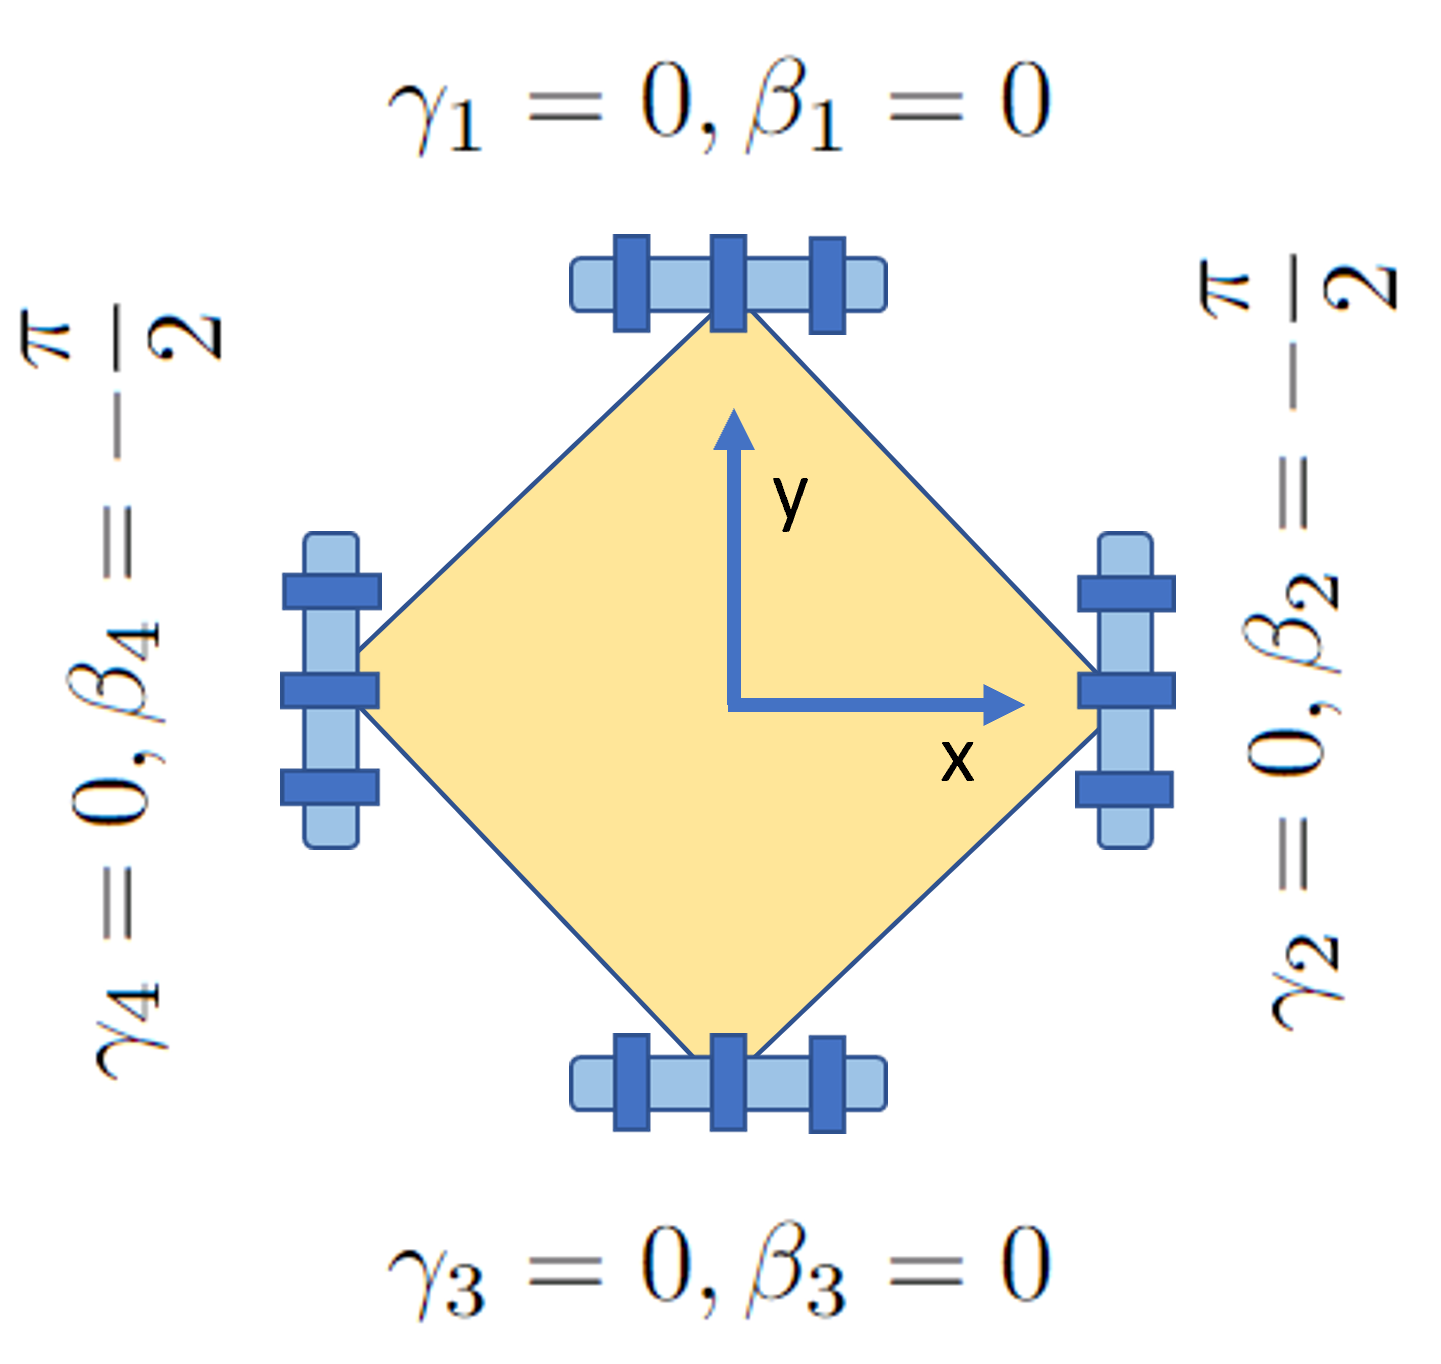
\includegraphics{robot_4_wheel_kinematics.png}\\

For wheel 1
\begin{align*}
    \gamma_1 = 0, \beta_1 = 0
\end{align*}

$y1 = -y3, x2 = -x4$

For wheel 2
\begin{align*}
    \gamma_2 = 0, \beta_2 = - \frac{\pi}{2}
\end{align*}

For wheel 3
\begin{align*}
    \gamma_3 = 0, \beta_3 = 0
\end{align*}

For wheel 4
\begin{align*}
    \gamma_4 = 0, \beta_4 =  -\frac{\pi}{2}
\end{align*}

\begin{equation}
    H(0)\mathcal{V}_b = \frac{1}{r}
    \begin{bmatrix}
        -y_1 & 1 & 0  \\
        -x_2 & 0 & -1 \\
        -y_3 & 1 & 0  \\
        -x_3 & 0 & -1 \\
    \end{bmatrix}
    \begin{bmatrix}
        \omega_{bz}   \\
        \upsilon_{bx} \\
        \upsilon_{by} \\
    \end{bmatrix}
\end{equation}

\begin{align}
    \mathcal{A} =
    \begin{bmatrix}
        -y_1 & 1 & 0  \\
        -x_2 & 0 & -1 \\
        -y_3 & 1 & 0  \\
        -x_3 & 0 & -1 \\
    \end{bmatrix}
\end{align}

\begin{align}
    \mathcal{A} =
    \begin{bmatrix}
        -y & 1 & 0  \\
        -x & 0 & -1 \\
        y & 1 & 0  \\
        x & 0 & -1 \\
    \end{bmatrix}
\end{align}

\section{For custom skateboard which is in our lab}

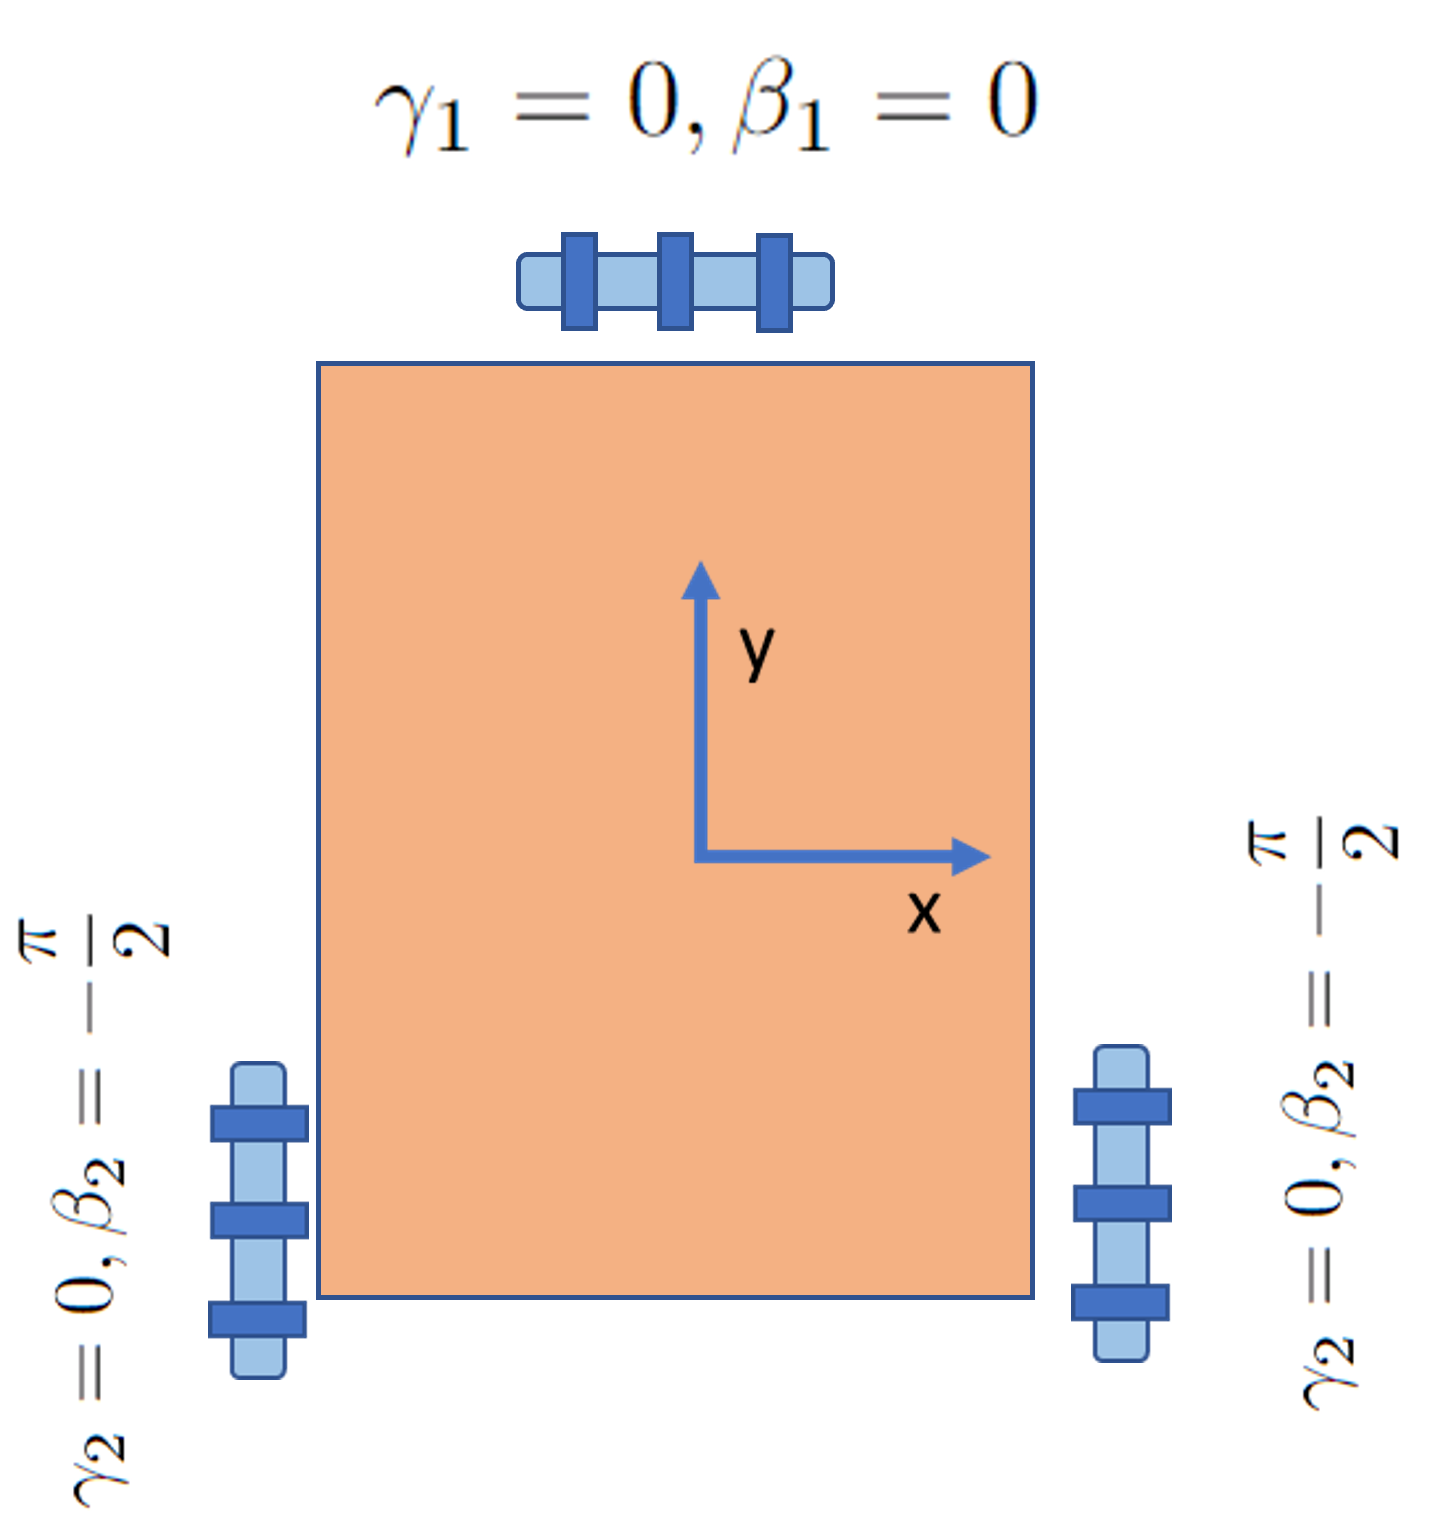
\includegraphics{custom_skateboard.png}

This is the same case of four wheel omnidirectional robot,
the resulant matrix will be

\begin{align}
    \mathcal{A} =
    \begin{bmatrix}
        -y_1 & 1 & 0  \\
        -x_2 & 0 & -1 \\
        -x_3 & 0 & -1 \\
    \end{bmatrix}
\end{align}

\begin{equation}
    H(0)\mathcal{V}_b = \frac{1}{r}
    \begin{bmatrix}
        -y_1 & 1 & 0  \\
        -x_2 & 0 & -1 \\
        -x_3 & 0 & -1 \\
    \end{bmatrix}
    \begin{bmatrix}
        \omega_{bz}   \\
        \upsilon_{bx} \\
        \upsilon_{by} \\
    \end{bmatrix}
\end{equation}

In case of $ y_1 = y, x_2 = -x_3$ the resultant matrix will be

\begin{equation}
    H(0)\mathcal{V}_b = \frac{1}{r}
    \begin{bmatrix}
        -y & 1 & 0  \\
        -x & 0 & -1 \\
        x & 0 & -1 \\
    \end{bmatrix}
    \begin{bmatrix}
        \omega_{bz}   \\
        \upsilon_{bx} \\
        \upsilon_{by} \\
    \end{bmatrix}
\end{equation}

% x hat
    $\hat{x}_b$
    

\end{document}